\section{Dijkstras Algoritme}
\begin{wrapfigure}{r}{0.45\textwidth}
    \centering
	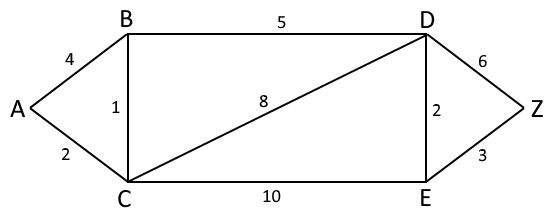
\includegraphics[width=0.45\textwidth]{Pictures/Teoriafsnit/Figurfiler/Graf.png}
	\label{fig:dijkstrasgraf}
	\caption{En vægtet graf}
\end{wrapfigure}

Dijkstra's er en grådig algoritme der kan finde en rute imellem to knudepunkter i en vægtet graf. I gruppens program er dette eksempelvis ruten mellem et køretøjs hjem og destination. Algoritmen starter med at sætte afstanden til alle punkter lig uendelig, udover start punktet da det er det eneste der kendes til på tidspunktet. Når algoritmen kører en graf igennem, kigger den på den node hvor kosten er lavest, og udregner kosten til de naboliggende noder. Når kosten udregnes for en nabo node, tages kosten af ruten til den nuværende node og afstanden til nabo noden bliver adderet. Da algoritmen altid tager noden med den lavest kost, vil den have fundet den korteste rute, når den nuværende node er slutnoden \cite[s. 681-684]{DMATBOGEN}. Som et eksempel kan vejen fra A til Z på figur \ref{fig:dijkstrasgraf} findes:

\begin{enumerate}
\item Algoritmen starter ved A, og kigger på naboerne B og C. Deres kost bliver noteret til at være 4 og 2.
\item Nu kigges der på noden C, da det er den nuværende korteste rute. Her ses det at kosten til B er 3 (2+1), og det bliver overskrevet da det er mindre end den tidligere værdi 4. Deruodver noteres det at kosten for D og E er 10 og 12.
\item Så kigges der på noden B, hvor det ses at kosten til D er 8 (2+1+5), og den overskriver den tidligere højere kost.
\item Derefter bliver noden D kigget på, hvor den noterer kosten for E og Z til at være 10 og 14. Selvom der er fundet en vej til slutnoden, forstættes der, da kosten til noden E er mindre end kosten til Z.
\item Så kigges der på noden E, hvor algoritmen ser at kosten til Z er 13, og dermed bliver den tidligere kost 14 overskrevet.
\item Der er ikke flere noder der har en lavere kost en slutnoden Z, og den korteste rute er fundet.
\end{enumerate}

Kostene for hver node kan gemmes i en tabel, som set på tabel \ref{dijktabel}.
	
\begin{table}[H]
\centering
	\begin{tabular}{|l|l|l|l|l|l|l|}
	\hline
	                 & A & B & C & D  & E  & Z  \\ \hline
	                 & 0 & $\infty$ & $\infty$ & $\infty$  & $\infty$  & $\infty$  \\ \hline
	A                & 0 & 4 & 2 & $\infty$  & $\infty$  & $\infty$  \\ \hline
	A, C             & 0 & 3 & 2 & 10 & 12 & $\infty$  \\ \hline
	A, C, B          & 0 & 3 & 2 & 8  & 12 & $\infty$  \\ \hline
	A, C, B, D       & 0 & 3 & 2 & 8  & 10 & 14 \\ \hline
	A, C, B, D, E    & 0 & 3 & 2 & 8  & 10 & 13 \\ \hline
	A, C, B, D, E, Z & 0 & 3 & 2 & 8  & 10 & 13 \\ \hline
	\end{tabular}
	\label{dijktabel}
	\caption{Dijkstra Kost Tabel}
\end{table}

\begin{figure}[H]
\begin{lstlisting}
Hmm...
\end{lstlisting}
\caption{Dijkstra pseudo-kode}\label{DijkstraCode}
\end{figure}